\documentclass{article}[12pt]

\usepackage[francais]{babel}
\usepackage{boxedminipage}
\usepackage[utf8]{inputenc}
\usepackage{amsfonts,amssymb,amsmath}
\usepackage[pdftex]{graphicx}
\usepackage{vmargin}

\usepackage{todonotes}

\usepackage{algorithm}
\usepackage[noend]{algpseudocode}
\usepackage{tcolorbox}

\newcommand*\Let[2]{\State #1 $\gets$ #2}
\algrenewcommand\algorithmicrequire{\textbf{Precondition:}}
\algrenewcommand\algorithmicensure{\textbf{Postcondition:}}

\newtcolorbox{mybox}[3][]
{
  colframe = #2!25,
  colback  = #2!10,
  coltitle = #2!20!black,  
  title    = {#3},
  #1,
}


\setpapersize{A4}
\setmarginsrb{2cm}{2cm}{2cm}{2cm}{0cm}{0cm}{0cm}{0cm} 

\setlength{\parindent}{0pt}

%\setlength{\textwidth}{17cm}
%\setlength{\evensidemargin}{0pt}
%\setlength{\oddsidemargin}{0pt}
%\setlength{\topmargin}{0pt}


\begin{document}
\begin{center}
\framebox[1.07\width]{
\begin{minipage}[b]{4cm}
%\includegraphics[width=4.5cm]{LOGO_EM.pdf}  
\end{minipage} 
\begin{minipage}[b]{11cm}
\ \\[.1cm]
%%%%%%%%%%%%%%%%%%%
%   ANNÉE 
Année 2021-2022
%%%%%%%%%%%%%%%%%%%
\hspace{\stretch{1}} 
%%%%%%%%%%%%%%%%%%%
% NUMERO DE SESSION
$2^\textrm{ème}$ session 
%%%%%%%%%%%%%%%%%%%
\\[.15cm]
\begin{center}
%%%%%%%%%%%%%%%%%%%
% DONNÉES DU MODULE
\textsc{Algorithmique et Structures de données}\\
\textsc{IF111}\\
\textsc{Rohan Fossé}\\
%%%%%%%%%%%%%%%%%%%
\end{center}
\ \\[.2cm]
%%%%%%%%%%%%%%%%%%%
% Données diverses
Filière : {T\'el\'ecom}
\hspace{\stretch{1}}
Année : {2021 - 2022}
\hspace{\stretch{1}}
Semestre : {1}
\\[.2cm]
Date de l'examen : {17 Mars 2022}
\hspace{\stretch{1}}
Durée de l'examen : {2h}
%%%%%%%%%%%%%%%%%%%
\\[.2cm]
\begin{tabular}{llll}
%%%%%%%%%%%%%%%%%%%
% remplacer $\Box$ par $\boxtimes$ pour cocher.
Documents autorisés &  $\Box$     & %\hspace{.5cm} &
sans document & $\boxtimes$ \\
Calculatrice autorisée & $\Box$ &
non autorisée & $\boxtimes$ \\
% remplacer $\Box$ par $\boxtimes$ pour cocher.
\end{tabular}
\\[.2cm]
%Autre : {.......}
\\[.2cm]
\end{minipage}
}

\end{center}

\vspace{1cm}
\begin{center}\huge{\textbf{SUJET}}\end{center}
\vspace{1cm}

%%%%%%%%%%%%%%%%%%%
% DÉBUT DU SUJET
%%%%%%%%%%%%%%%%%%%

\begin{center}
  \begin{boxedminipage}{\linewidth}
    {\large {\bf Nom et Prénom} :}~\\
  \end{boxedminipage}
\end{center}

\textbf{
\begin{itemize}
\item Toutes les parties du sujet sont indépendantes (en particulier les exercices) ;
\item Il est impératif de répondre dans les espaces prévus à cet effet : ce qui dépasse
  ne sera pas lu. Pour les parties où il faut écrire du code, merci d'écrire une ligne
  devant chaque numéro. \textbf{Vous êtes donc limités dans la quantité de code que vous êtes
  autorisés à écrire pour chaque question.}
\item Merci d'écrire dans un français correct : orthographe, grammaire et conjugaison
  seront pris en compte dans la correction ;
\item Vos codes doivent être indentés correctement ;
\item Le barême est donné à titre indicatif ;
\item Merci de retirer les pages d'annexe du sujet avant de rendre votre copie ;
\item Enfin, n'oubliez pas d'indiquer votre NOM sur la copie !
\end{itemize}
}

\section*{Exercice 1}
Pour chacune des fonctions suivantes, déterminer la complexité asymptotique dans la notation $\mathcal{O}$.
\begin{tcolorbox}
\begin{enumerate}
    \item $T_1(n) = 2n^5 + 10n^2 - 2n^4 + 10$
    \item $T_2(n) = 3log_2(n) + 4$
    \item $T_3(n) = 4log_2n + n$
    \item $T_4(n) = 15k + 3$
    \item $T_5(n) = 2^n + 20n^2 + 7$
    \item $T_6(n) = 2log_{10}k + kn^2$
\end{enumerate}
\end{tcolorbox}


\newpage
\section*{Exercice 2}
  Calculer la complexité asymptotique dans la notation $\mathcal{O}$ de la fonction \textit{mystère} suivante:
  
  
  \begin{tcolorbox}
         \begin{algorithmic}[1]
    \Function{$mystere$}{$n$}
    \Let{$m$}{0}
    \Let{$i$}{0}
    \Let{$j$}{0}
    \For{$i < n$}
        \For{$j < i$}
            \Let{$m$}{$ m * i * j + 1$}
        \EndFor
    \EndFor
  \EndFunction
  \end{algorithmic}
\end{tcolorbox}


\section*{Exercice 3}

Dans cet exercice, on considère un graphe pondéré. Appliquer l'algorithme de Dijkstra au graphe dans la Figure ci-dessous pour calculer la plus courte distance de $A$ à $D$.

\begin{figure}[h!] 
  \centering
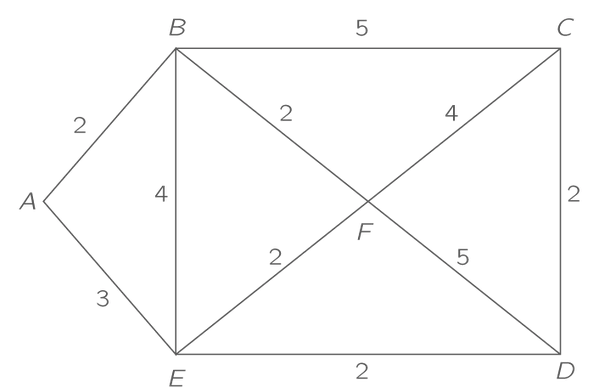
\includegraphics[scale =0.3]{Djikstra.png} \label{fig:grapheDijkstra}
\end{figure}


\section*{Exercice 4}

Tout graphe contenant un triangle ($K_3$) ne peut être colorié en moins de trois couleurs.

\begin{enumerate}
    \item Construire un graphe sans triangle qui nécessite également trois couleurs.
    \item Comment construire un graphe sans $K_4$ nécessitant 4 couleurs ?
    \item Un graphe sans $K_5$ nécessitant 5 couleurs ?
\end{enumerate}



\section*{Exercice 5}
Écrivez les fonctions suivantes sur les listes en utilisant les fonctions données ci-dessous:

\begin{itemize}
    \item $vide(l)$ : Renvoie $True$ si la liste $l$ est vide et $False$ sinon;
    \item $cons(a,l)$: Renvoie la liste obtenue en ajoutant l'élément $a$ devant la liste $l$;
    \item $tete(l)$: Renvoie le premier élément de la liste $l$;
    \item $queue(l)$ Renvoie la queue de la liste, ie $l$ sans le premier élément.
\end{itemize}


\begin{enumerate}
    \item $le\_plus\_souvent(x,l)$ qui renvoie $True$ si l’élément $x$ apparaît le plus de fois dans la liste $l$ et $False$ sinon;
    \item $millieme(l)$ qui renvoie le millième élément de la liste $l$ (on suppose que la liste l a au moins
mille éléments donc il n’est pas nécessaire de traiter le cas d’erreur);
    \item $facto\_liste(l)$ qui renvoie la liste contenant la factorielle de chacun des éléments de la liste $l$
(si l contient les valeurs 4, 3 et 2, la fonction doit renvoyer une liste contenant les valeurs 24, 6 et
2) ;
    \item $diff(l1,l2)$ qui renvoie la liste contenant la différence des éléments de $l_1$ et $l_2$. On suppose que la liste $l_1$ est de taille supérieure ou égale à la liste $l_2$ (si $l_1$ contient les entiers 4, 5 et 6 et $l_2$ contient les entiers 1 et 2, la fonction doit renvoyer une liste contenant les valeurs 3, 3 et 6) ;
    \item $double(l)$ qui renvoie True si chaque élément de la liste est supérieur au double de son prédécesseur, et $False$ sinon (par exemple sur la liste 2, 5, 10 et 23 la fonction renverra $True$ mais sur la liste 2, 4, 9, 12 et 25 elle renverra $False$ car 12 est inférieur au double de 9) ;

\end{enumerate}

\section*{Exercice 6}

On veut concevoir des algorithmes récursifs pour calculer des propriétés d'un arbre binaire donné en entrée. 
Ces algorithmes pourront utiliser les fonctions suivantes: 
\begin{itemize}
    \item $estVide(T)$ qui retourne vrai si l'arborescence $T$ est vide
    \item $filsGauche(T)$ et $filsDroit(T)$ qui retournent respectivement le sous-arbre gauche et le sous-arbre droit de l'arbre $T$.
\end{itemize}

 Décrire brièvement le fonctionnement des algorithmes suivants et en écrire le pseudo-code.
\begin{enumerate}			
\item Concevoir un algorithme récursif, nommé $hauteur(T)$, qui calcule la hauteur d'une arborescence binaire $T$ donnée en entrée. Si l'arborescence est vide l'algorithme retournera $-1$.

\item Concevoir un algorithme récursif, nommé $nombreFeuilles(T)$, qui calcule le nombre de feuilles d'une arborescence binaire $T$ donnée en entrée. 
\end{enumerate}	
	
	
\section*{Exercice 7}

Considérons le graphe $G$ suivant:\\

\begin{figure}[h!]
    \centering
    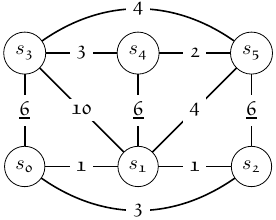
\includegraphics{Kruskal-1.png}
    \label{fig:my_label}
\end{figure}

Appliquer l'algorithme de \textit{Prim} pour trouver un arbre couvrant de poids minimum au graphe $G$.
\end{document}

